
\section{Debugging and Profiling}
In sequential programming measuring the performance of a program can be done through measuring its execution time.
This can be acheived by recording the time when the program starts and when it finishes, and calculating the difference.

However, in concurrent processing, execution times of individual instructions may overlap, making it challenging to calculate the execution time of the individual instructions \cite[21]{volkovLatencyHiding2016}.

Two commonly used metrics for measuring the performance of concurrent programs are throughput and latency. Latency refers to the average time taken between the start and end of a task, while throughput represents the amount of work performed per unit of time \cite[21-23]{volkovLatencyHiding2016}.


\subsection{Creating Minimal Testing Example}


Wen debugging and profiling real-time applications it is often b

Beyond this the use of coroutines offers more control over the execution of the program, at the cost of requiring more thought to be put into the design of the program to avoid blocking the event loop.

\subsubsection{Python Profilers}
While none of the following profiling methods offer a complete insight into the performance of asynchronous \py programs, they are useful for identifying bottlenecks and frequently scheduled coroutines.

The built-in Python profiler, \code{CProfile}, can be used to measure the execution time of individual functions and the number of times they are called \cite{pythonsoftwarefoundationPythonProfilers}.
It is particularly helpful in identifying slow-running functions, and visualization tools like SnakeViz can be used to analyze the collected information \cite{davisSnakeViz2023}.
Another valuable tool is the \code{line_profiler} package, which provides a line-by-line profiler for identifying slow lines of code \cite{kernLineProfilerKernprof2023}.

Other tools, such as the \code{austin} plugin for \gls{vscode}, were tested but ultimately discarded as they did not perform as effectively as the previous two methods \cite{tornettaAustinVSCode2023}.


\subsection{Nsight Systems}
Nsight is a suite of tools for debugging and profiling CUDA applications.
Three tools have been used for debugging and profiling during the \gls{cuda} code presented in Chapter \label{chap:debayer}.
The \code{Nsight for Visual Studio} plugin for \gls{vscode} enables the use of breakpoints and step-by-step debugging in \gls{cuda} kernels \cite{nvidiaNsightVisualStudio2021}.
As \gls{cuda} code is executed in parallel this does not always offer the same level of insight as when debugging sequential code, but it can still be useful for identifying errors in the code.

For profiling, the \code{nsys profile} command line tool has been used.
It can be used to collect a wide range of information about the execution of a program, including the execution time of individual kernels, memory usage
\footnote{On the \jx, profiling memory the use of Pinned Memory appear to be broken.}
, and the number of times each cuda related function is called \cite{nvidiaNVIDIANsightSystems2023}.

The \code{nsys profile} tool can also export the collected information to a \code{sqlite} database, which can be visualized using the \code{Nsight Compute} \gls{gui} \cite{nvidiaNVIDIANsightSystems2023}.
A zoomed out view of the timeline can be seen in Figure \ref{fig:nsight_compute_timeline}.


\subsection{Nsight Compute}
\begin{figure}[H]
    \centering
    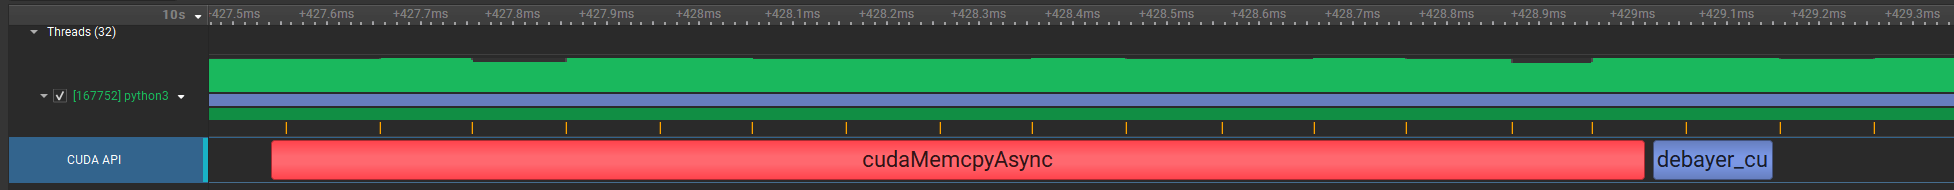
\includegraphics[width=\textwidth]{figures/memory_comparaison.png}
    \caption{Screenshot of Nsight Compute during profiling the kernel presented in Chapter \ref{chap:debayer}.}
    \label{fig:}
\end{figure}


% \begin{listing}[H]
%     \begin{minted}{python}
%         import asyncio, threading, time

%         def do_nothing(): pass
%         async def do_nothing_async(): pass

%         async def test_asyncio():
%             start_time = time.perf_counter()
%             await asyncio.gather(*[do_nothing_async() for _ in range(10000)])
%             end_time = time.perf_counter()
%             print(f"Asyncio took {end_time - start_time:.6f} seconds to complete.")

%         def test_threads():
%             threads = [threading.Thread(target=do_nothing) for _ in range(10000)]
%             start_time = time.perf_counter()
%             for thread in threads:
%                 thread.start()
%             for thread in threads:
%                 thread.join()
%             end_time = time.perf_counter()
%             print(f"Threads took {end_time - start_time:.6f} seconds to complete.")

%         if __name__ == "__main__":
%             asyncio.run(test_asyncio())
%             test_threads()
%     \end{minted}
%     \begin{minted}{bash}
%         >>> Asyncio took 0.311703 seconds to complete.
%         >>> Threads took 11.898036 seconds to complete.
%     \end{minted}
%     \caption{Comparison of asyncio and threads running on INTEL i7-11800H @ 2.30GHz.}
% \end{listing}